% -*- latex -*-
%%%%%%%%%%%%%%%%%%%%%%%%%%%%%%%%%%%%%%%%%%%%%%%%%%%%%%%%%%%%%%%%
%%%%%%%%%%%%%%%%%%%%%%%%%%%%%%%%%%%%%%%%%%%%%%%%%%%%%%%%%%%%%%%%
%%%%
%%%% This text file is part of the source of
%%%% `Parallel Programming in MPI and OpenMP'
%%%% by Victor Eijkhout, copyright 2012-2024
%%%%
%%%% omp-sync.tex : synchronization
%%%%
%%%%%%%%%%%%%%%%%%%%%%%%%%%%%%%%%%%%%%%%%%%%%%%%%%%%%%%%%%%%%%%%
%%%%%%%%%%%%%%%%%%%%%%%%%%%%%%%%%%%%%%%%%%%%%%%%%%%%%%%%%%%%%%%%

\index{synchronization!in OpenMP|(}

In the constructs for declaring parallel regions above, you had little control over 
in what order threads executed the work they were assigned.
This section will discuss \emph{synchronization} constructs: ways of telling
threads to bring a certain order to the sequence in which they do things.

\begin{itemize}
\item \texttt{critical}: a section of code can only be executed by one
  thread at a time; see~\ref{sec:critical}.
\item \texttt{atomic} \emph{Atomic update}\index{atomic operation}
  of a single memory location. Only certain
  specified syntax patterns are supported. This was added in order to
  be able to use hardware support for atomic updates.
\item \texttt{barrier}: section~\ref{sec:ompbarrier}.
\item locks: section \ref{sec:ompref:locks}.
\item \texttt{flush}: section \ref{sec:omp:flush}.
\end{itemize}
Loop-related synchronization constructs were discussed earlier:
\begin{itemize}
\item \texttt{ordered}: section~\ref{sec:omp-ordered}.
\item \texttt{nowait}: section~\ref{sec:omp-nowait}.
\end{itemize}

\Level 0 {Barrier}
\label{sec:ompbarrier}

A \indexompdef{barrier} defines a point in the code where all active threads will stop
until all threads have arrived at that point. With this, you can guarantee that
certain calculations are finished. For instance, in this code snippet, computation 
of~\n{y} can not proceed until another thread has computed its value of~\n{x}.
\begin{lstlisting}
#pragma omp parallel 
{
  int mytid = omp_get_thread_num();
  x[mytid] = some_calculation();
  y[mytid] = x[mytid]+x[mytid+1];
}
\end{lstlisting}
This can be guaranteed with a \indexpragma{barrier} pragma:
\begin{lstlisting}
#pragma omp parallel 
{
  int mytid = omp_get_thread_num();
  x[mytid] = some_calculation();
#pragma omp barrier
  y[mytid] = x[mytid]+x[mytid+1];
}
\end{lstlisting}

\Level 1 {Implicit barriers}
\label{sec:ompbarrierimpl}

Apart from the barrier directive, which inserts an explicit barrier,
OpenMP has \emph{implicit barriers}\index[omp]{omp!barrier!implicit} after
a work sharing construct; see section~\ref{sec:omp-single}.
Thus the following code is well defined:
\begin{lstlisting}
#pragma omp parallel 
{
#pragma omp for
  for (int mytid=0; mytid<number_of_threads; mytid++)
    x[mytid] = some_calculation();
#pragma omp for
  for (int mytid=0; mytid<number_of_threads-1; mytid++)
    y[mytid] = x[mytid]+x[mytid+1];
}
\end{lstlisting}

You can also put each parallel loop in a parallel region of its own,
but there is some overhead associated with creating and deleting the
team of threads in between the regions.

At the end of a parallel region the team of threads is dissolved and
only the master thread continues. Therefore, there is an
\emph{implicit barrier at the end of a parallel region}%
\index[omp]{parallel region!barrier at the end of}.
This barrier behavior can be canceled with the \indexclause{nowait}
clause.

You will often see the idiom
\begin{lstlisting}
#pragma omp parallel
{
#pragma omp for nowait
  for (i=0; i<N; i++)
    a[i] = // some expression
#pragma omp for
  for (i=0; i<N; i++)
    b[i] = ...... a[i] ......
\end{lstlisting}
Here the \n{nowait} clause implies that threads can start on the second loop
while other threads are still working on the first. Since the two loops use the same
schedule here, an iteration that uses \n{a[i]} can indeed rely on it that that 
value has been computed.

\Level 0 {Mutual exclusion}

Sometimes it is necessary to limit a piece of code
so that it can be executed by only one tread at a time.
Such a piece of code is called a \indexterm{critical section}, and
OpenMP has several mechanisms for realizing this.

\Level 1 {Race conditions}

OpenMP, being based on shared memory, has a potential for
\emph{race conditions}.
These happen when two threads access the same data
item, with at least one access a write.
The problem with race conditions is that programmer convenience
runs counter to efficient execution.

For a simple example:
%\csnippetwithoutput{racecounter}{racecounter}
\csnippetwithoutput{racecounter}{examples/omp/c}{race}

The basic rule about multiple-thread access of a single data item is:
\begin{quote}
  Any memory location that is \emph{written} by one thread, can not be
  \emph{read} by another thread in the same parallel region, if no
  synchronization is done.
\end{quote}

To start with that last clause: any workshare construct ends with an
\indextermsub{implicit}{barrier}, so data written before that barrier
can safely be read after it.

\Level 1 {\texttt{critical} and \texttt{atomic}}
\label{sec:critical}
\index{atomic operation!OpenMP|(}

There are two pragmas for critical sections: \indexpragma{critical} and \indexpragma{atomic}.
Both denote \emph{atomic operations}
in a technical sense.
The first one is general and can contain an arbitrary sequence of instructions;
the second one is more limited but has performance advantages.

Beginning programmers are often tempted to use \indexpragma{critical}
for updates in a loop:
\begin{lstlisting}
#pragma omp parallel
{
  int mytid = omp_get_thread_num();
  double tmp = some_function(mytid);
  // This Works, but Not Best Solution:
#pragma omp critical
  sum += tmp;
}
\end{lstlisting}
but this should really be done with a \indexpragma{reduction} clause,
which will be far more efficient.

\begin{figure}[ht]
  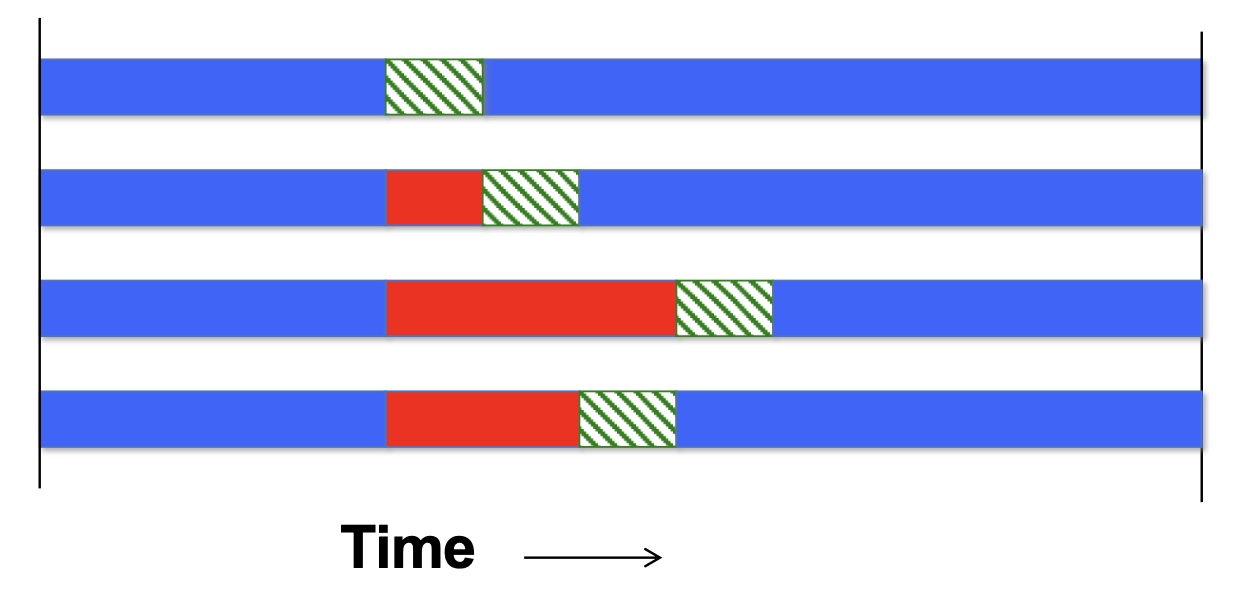
\includegraphics{omp-idle}
  \caption{Idle time induced by a critical section}
  \label{fig:omp-idle}
\end{figure}
Figure~{fig:omp-idle} illustrates how a critical section induces idle time:
threads have to wait at the initial barrier
until its their turn to enter the critical section.
In effect, the execution becomes sequential!

A good use of critical sections is doing file writes or database updates.

\begin{exercise}
  Consider  a loop where each iteration updates a variable.
\begin{lstlisting}
#pragma omp parallel for shared(result)
  for ( i ) {
      result += some_function_of(i);
  }
\end{lstlisting}
  Discuss qualitatively
  the difference between:
  \begin{itemize}
  \item  turning the update statement into a critical section, versus
  \item letting the threads accumulate into a private variable \n{tmp} as above,
    and summing these after the loop.
  \end{itemize}  
  Do an Ahmdal-style quantitative analysis of the first case, assuming
  that you do $n$ iterations on $p$ threads, and each iteration has a
  critical section that takes a fraction~$f$.  Assume the number of
  iterations~$n$ is a multiple of the number of threads~$p$. Also
  assume the default static distribution of loop iterations over the
  threads.
\end{exercise}

Critical sections are an easy way to turn an existing code into a correct parallel code.
However, there are performance disadvantages to critical sections,
and sometimes a more drastic rewrite
is called for.

A critical section works by acquiring a lock, which carries a substantial overhead.
Furthermore, if your code has multiple critical sections, they are all mutually exclusive:
if a thread is in one critical section, the other ones are all blocked.

The problem with \n{critical} sections being mutually exclusive can be mitigated by naming them:
\begin{lstlisting}
#pragma omp critical (optional_name_in_parens)
\end{lstlisting}

On the other hand, the syntax for \n{atomic} sections is limited to the update
of a single memory location, but such sections
are not exclusive and they can be more efficient, since they assume that there is a hardware
mechanism for making them critical. See the next section.

\Level 1 {\texttt{atomic} construct}
\label{sec:atomic}

While the \indexclause{critical} construct can enclose arbitrary blocks of code,
the \indexompclause{atomic} clause has one of a limited number of forms,
for which hardware support is likely.
Those consist of assigning to a variable:
\begin{lstlisting}
x++;
// or:
x += y;
\end{lstlisting}
possibly combination with reading that variable:
\begin{lstlisting}
v = x; x++;
\end{lstlisting}

There are various further refinements on the atomic specification:
\begin{enumerate}
\item \lstinline{omp atomic write} is followed by  a single assignment statement
  to a shared variable.
\item \lstinline{omp atomic read} is followed by  a single assignment statement
  from a shared variable.
\item \lstinline{omp atomic} is equivalent to \lstinline{omp atomic update};
  it accomodates statements such as 
  \begin{lstlisting}
    x++; x += 1.5;
  \end{lstlisting}
\item \lstinline{omp atomic capture} can accommodate a single statement
  similar to \lstinline{omp atomic update},
  or a block that essentially combines a \lstinline{read} and \lstinline{update} form.
\end{enumerate}

\index{atomic operation!OpenMP|)}

\Level 0 {Locks}
\index{lock|(textbf}
\label{sec:ompref:locks}

OpenMP also has the traditional mechanism of a \indexterm{lock}. A~lock is somewhat similar to 
a critical section: it guarantees that some instructions can only be performed by one
process at a time. However, a critical section is indeed about code; a~lock is about data.
With a lock you make sure that some data elements can only be touched by one process at a time.

\Level 1 {Routines}

Create/destroy:
\begin{lstlisting}
void omp_init_lock(omp_lock_t *lock);
void omp_destroy_lock(omp_lock_t *lock);
\end{lstlisting}
Set and release:
\begin{lstlisting}
void omp_set_lock(omp_lock_t *lock);
void omp_unset_lock(omp_lock_t *lock);
\end{lstlisting}
Since the set call is blocking, there is also 
\begin{lstlisting}
int omp_test_lock();
\end{lstlisting}
which returns true if the lock was successfully set;
otherwise it return false and continues execution with the next statement.

Unsetting a lock needs to be done by the thread that set it.

Lock operations implicitly have a \indexpragma{flush};
see section \ref{sec:omp:flush}.

\begin{exercise}
  \label{ex:loc-deadlock}
  %% https://computing.llnl.gov/tutorials/openMP/samples/C/omp_bug5.c
  %% I think this is fundamentally broken
  In the following code, one process sets array~A and then uses it to
  update~B; the other process sets array~B and then uses it to
  update~A.
  Argue that this code can deadlock. How could you fix this?
\begin{lstlisting}
#pragma omp parallel shared(a, b, nthreads, locka, lockb)
  #pragma omp sections nowait
    {
    #pragma omp section
      {
      omp_set_lock(&locka);
      for (i=0; i<N; i++)
        a[i] = ..

      omp_set_lock(&lockb);
      for (i=0; i<N; i++)
        b[i] = .. a[i] ..
      omp_unset_lock(&lockb);
      omp_unset_lock(&locka);
      }

    #pragma omp section
      {
      omp_set_lock(&lockb);
      for (i=0; i<N; i++)
        b[i] = ...

      omp_set_lock(&locka);
      for (i=0; i<N; i++)
        a[i] = .. b[i] ..
      omp_unset_lock(&locka);
      omp_unset_lock(&lockb);
      }
    }  /* end of sections */
  }  /* end of parallel region */
\end{lstlisting}
\end{exercise}

\Level 1 {Example: Mandelbrot set}

Section \ref{sec:omp-mandel-oracle} has an approach to the  \indexterm{Mandelbrot set}
based locking a FIFO that has the coordinates to be processed.

\Level 1 {Example: object with atomic update}

\ac{OO} languages such as C++ allow for syntactic simplification,
for instance building the locking and unlocking actions into
the update operator.

\begin{cppnote}{Lock inside overloaded operator}
  \label{cpp:op-lock}
  \cverbatimsnippet[examples/omp/cxx/lockobject.cxx]{lockobject}

  Running this:

  \cverbatimsnippet[examples/omp/cxx/lockobject.cxx]{lockobjectuse}
\end{cppnote}

\Level 1 {Example: histogram / binning}

One simple example of the use of locks is generation of a \indexterm{histogram}
(also known as the \emph{binning}\index{binning|see{histogram}} problem).
A~histogram consists of a number of bins, that get updated depending on some data.
Here is the basic structure of such a code:
\begin{lstlisting}
int count[100];
float x = some_function();
int ix = (int)x;
if (ix>=100)
  error();
else
  count[ix]++;
\end{lstlisting}
It would be possible to guard the last line:
\begin{lstlisting}
#pragma omp critical
  count[ix]++;
\end{lstlisting}
but that is unnecessarily restrictive. If there are enough bins in the
histogram, and if the \n{some_function} takes enough time, there are unlikely to be
conflicting writes. The solution then is to create an array of locks, with
one lock for each \n{count} location.

Another solution would be to give each thread a local copy
of the result array, and perform a reduction on these.
See section~\ref{sec:omp-array-reduct}.

\Level 1 {Nested locks}

A lock as explained above can not be locked if it is already locked.
A~\indextermsub{nested}{lock} can be locked multiple times by the same
thread before being unlocked.

\begin{itemize}
\item \indexompdef{omp_init_nest_lock}
\item \indexompdef{omp_destroy_nest_lock}
\item \indexompdef{omp_set_nest_lock}
\item \indexompdef{omp_unset_nest_lock}
\item \indexompdef{omp_test_nest_lock}
\end{itemize}

\index{lock|)}

\Level 0 {Relaxed memory model}
\label{sec:omp:flush}

\indexpragma{flush}

\begin{itemize}
\item There is an implicit flush of all variables at the start and end 
  of a \emph{parallel region}\index{parallel region!flush at}.
\item There is a flush at each barrier, whether explicit or implicit,
  such as at the end of a
  \emph{work sharing}\index{workshare!flush after}.
\item At entry and exit of a
  \emph{critical section}\index{critical section!flush at}
\item When a \emph{lock}\index{lock!flush at} is set or unset.
\end{itemize}

\Level 0 {Example: Fibonacci computation}
\index{Fibonacci sequence|(}

The \emph{Fibonacci sequence} is recursively defined as
\[ F(0)=1,\qquad F(1)=1,\qquad F(n)=F(n-1)+F(n-2)
\hbox{ for $n\geq2$}.
\]
We start by sketching the basic single-threaded solution.
The naive code looks like:
\begin{lstlisting}
int main() {
  value = new int[nmax+1];
  value[0] = 1;
  value[1] = 1;
  fib(10);
}

int fib(int n) {
  int i, j, result;
  if (n>=2) {
    i=fib(n-1); j=fib(n-2);
    value[n] = i+j;
  }
  return value[n];
}
\end{lstlisting}
However, this is inefficient, since most intermediate values will be computed
more than once. We solve this by keeping track of which results are known:
\begin{lstlisting}
  ...
  done = new int[nmax+1];
  for (i=0; i<=nmax; i++)
    done[i] = 0;
  done[0] = 1;
  done[1] = 1;
  ...
int fib(int n) {
  int i, j;
  if (!done[n]) {
    i = fib(n-1); j = fib(n-2);
    value[n] = i+j; done[n] = 1;
  }
  return value[n];
}
\end{lstlisting}
The OpenMP parallel solution calls for two different ideas. First of all,
we parallelize the recursion by using tasks (section~\ref{sec:omp:task}:
\begin{lstlisting}
int fib(int n) {
  int i, j;
  if (n>=2) {
#pragma omp task shared(i) firstprivate(n)
    i=fib(n-1);
#pragma omp task shared(j) firstprivate(n)
    j=fib(n-2);
#pragma omp taskwait
    value[n] = i+j;
  }
  return value[n];
}
\end{lstlisting}
This computes the right solution, but, as in the naive single-threaded solution,
it recomputes many of the intermediate values.

A naive addition of the \n{done} array leads to data races, and probably an
incorrect solution:
\begin{lstlisting}
int fib(int n) {
  int i, j, result;
  if (!done[n]) {
#pragma omp task shared(i) firstprivate(n)
    i=fib(n-1);
#pragma omp task shared(i) firstprivate(n)
    j=fib(n-2);
#pragma omp taskwait
    value[n] = i+j;
    done[n] = 1;
  }
  return value[n];
}
\end{lstlisting}
For instance, there is no guarantee that the \n{done} array is updated
later than the \n{value} array, so a thread can think that \n{done[n-1]}
is true, but \n{value[n-1]} does not have the right value yet.

One solution to this problem is to use a lock, and make sure that,
for a given index~\n{n}, the values \n{done[n]} and \n{value[n]}
are never touched by more than one thread at a time:
\begin{lstlisting}
int fib(int n)
{
  int i, j;
  omp_set_lock( &(dolock[n]) );
  if (!done[n]) {
#pragma omp task shared(i) firstprivate(n)
    i = fib(n-1);
#pragma omp task shared(j) firstprivate(n)
    j = fib(n-2);
#pragma omp taskwait
    value[n] = i+j;
    done[n] = 1;
  }
  omp_unset_lock( &(dolock[n]) );
  return value[n];
}
\end{lstlisting}
This solution is correct, optimally efficient in the sense that it
does not recompute anything, and it uses tasks to obtain a parallel execution.

However, the efficiency of this solution is only up to a constant.
A~lock is still being set, even if a value is already computed and therefore
will only be read. This can be solved with a complicated use of critical sections,
but we will forego this.

\index{Fibonacci sequence|)}

\index{synchronization!in OpenMP|)}

